%!TEX TS-program = xetex
\documentclass{TDP005mall}
\usepackage[utf8]{inputenc}
\usepackage[swedish]{babel}
\usepackage[export]{adjustbox}
\usepackage{tabularx}
\usepackage{caption}

\usepackage[style=authoryear, backend=biber]{biblatex}
\usepackage{filecontents}
\begin{filecontents}{reference.bib}
@online{grotto1,
author="ansimuz",
title="Platform Pixel Art Assets",
howpublished ="Website",
date = "2015-02-05",
url ="https://opengameart.org/content/platform-pixel-art-assets",
urldate="2020-11-24",
}
@online{grotto2,
author="ansimuz",
title="Grotto Escape II - Environment",
howpublished ="Website",
date = "2017-01-08",
url ="https://opengameart.org/content/grotto-escape-ii-environment",
urldate="2020-11-24",
}
\end{filecontents}
\addbibresource{reference.bib}
\usepackage{csquotes}

\renewcommand*{\contentsname}{Innehållsförteckning}

\newcommand{\version}{Version 1.1}
\author{Daniel Huber, \url{danhu849@student.liu.se}\\
  Viktor Rösler, \url{vikro653@student.liu.se}}
\title{Kravspecifikation}
\date{2020-11-28}
\rhead{Daniel Huber\\
Viktor Rösler}

% For aligning captions to the left.
\captionsetup{justification=raggedright,singlelinecheck=false} 

\begin{document}
\projectpage
\tableofcontents
\newpage
\section{Revisionshistorik}
\begin{table}[!h]
\begin{tabularx}{\linewidth}{|l|X|l|}
\hline
  Ver. & Revisionsbeskrivning & Datum \\\hline
    1.1 & Kompletering och kravuppfyllelse & 201128 \\\hline
1.0 & Kravspecifikation TDP005 & 201127 \\\hline
\\\hline
\end{tabularx}
\end{table}


\section{Spelid\'{e} }
% Vad går spelet ut på? - Tänk: vad ska stå på Steam-sidan som säljer ert spel?
Din familj har kidnappads av Ondskan! Du vet om att Ondskan håller till på toppen av ett berg omgivet av lava, men du vet inte vilket! Hoppa upp på plattformarna, undvik den ökande nivån av lava, döda eller undvik fienderna och ta dig uppför berget så snabbt som möjligt! I denna bottom-top platformsscroller kan du spela ensam eller tillsammans med en vän. Kan du rädda din familj? 

\subsection{Spelets mål}
Varje nivå avklaras när toppen av nivån nås av spelaren. Spelet ses vara avklarat när toppen på den sista nivån nås. På vägen upp mot toppen dödas eller undviks fiender. 

\section{Målgrupp}% Vilka typer av spelare borde spela ert spel?
Spelet riktas mot spelare som underhålls av spel med stegrande utmaning för varje nivå och där nivåer måste avklaras under en viss tidspress. 

\section{Spelupplevelse}% Vad gör spelet underhållande att spela?
Spelaren tvingas i varje nivå hitta den mest tidseffektiva vägen upp samtidigt som fiender måste undvikas eller dödas. Vid spelets målgång belönas spelaren med en känsla av tillfredställelse över att ha klarat av en utmaning då spelet designats att vara svårt.

\subsection{Multiplayer}
Multiplayer kan aktiveras för att möjliggöra lokalt spel för två spelare. Vid den ena spelarens död kan den andre spelaren fortsätta nivån. Antingen hjälps spelare åt att klara nivåerna eller så kan friendly-fire aktiveras för att öka svårighetsgraden ytterligare då spelarna skadas av den andres projektiler.

\section{Spelmekanik}% Hur interagerar man med spelet? Vilka kommandon? Vad driver spelet framåt?
Nivåerna startas med spelarkaraktären vid botten av berget med tre liv och en pistol. Efter att första plattformen nås börjar lavan stiga. Genom nivån följs spelaren av spelarfönstret. I takt med att spelaren rör sig uppåt syns fler platformar spelaren kan hoppa upp till. På plattformar dödas eller undviks fiender av spelaren. Mellan platformar kan flygande fiender finnas. Spelarens väg upp mot toppen försvåras av att platformar inte kan hoppas igenom. Game over triggas om spelaren skadas till noll liv.
\newpage
\subsection{Förflyttning} % Lägga in tabell för xbox kontroll förflyttning.

\begin{table}[h!]
  \caption{Tangentbordskommandon\label{tab:1}}
\begin{tabular}{|l|l|}
\hline
Tangent & Resultat \\\hline
↑, Z & Spelaren hoppar uppåt. \\\hline
← & Spelaren förflyttas åt vänster. \\\hline
→ & Spelaren förflyttas åt höger. \\\hline
↑ + ←, Z + ← & Spelaren hoppar åt vänster. \\\hline
↑ + →, Z + → & Spelaren hoppar åt höger. \\\hline
X & Ett skott avfyras i den riktningen spelaren är vänd åt. \\\hline
\end{tabular}
\end{table}

\begin{table}[h!]
  \caption{Handkontrollskommandon (Xbox 360)\label{tab:2}}
\begin{tabular}{|l|l|}
\hline
Knapp & Resultat \\\hline
A & Spelaren hoppar uppåt. \\\hline
Vänster styrspak lutad åt vänster.  & Spelaren förflyttas åt vänster. \\\hline
Vänster styrspak lutad åt höger. & Spelaren förflyttas åt höger. \\\hline
A + Vänster styrspak lutad åt vänster. & Spelaren hoppar åt vänster. \\\hline
A + Vänster styrspak lutad åt höger. & Spelaren hoppar åt höger. \\\hline
Höger avtryckare & Ett skott avfyras i den riktningen spelaren är vänd åt. \\\hline
\end{tabular}
\end{table}

Spelaren styrs med hjälp av antingen tangentbordet enligt tabell \ref{tab:1} eller en Xbox 360 handkontroll enligt tabell \ref{tab:2}. I luften styrs spelaren av respektive riktningskommando. Spelare kan förflyttas i både vänster-, höger- och höjdled med hjälp av hopp. Det finns bara en fixerad hopphöjd. Vid kontinuerlig rörelse åt något håll byggs momentum upp och spelarkaraktären förflyttas ytterligare en liten bit i förflyttningsriktningen när spelarinput slutat ges.

\subsection{Fiender}
Över nivåerna förflyttas fiender i förutbestämda mönster. De finns på platformar eller i luften mellan platformarna. Det ges ingen visuell representation i spelet av hur många återstående liv en fiende har. Tre typer av fiender finns.

\subsubsection*{Flygande fiende 1}
\begin{figure}[h!]
  \caption{Flygande fiende 1\label{fig:1}}
  
\includegraphics[height=1.5cm]{/home/danhu849/tdp005/Documents/images/sflying_enemy1.png}
\end{figure}

\begin{table}[h!]
  \caption{Egenskaper: Flygande fiende 1\label{tab:3}}
\begin{tabular}{|l|l|}
\hline
Attribut & Värde \\\hline
Liv & 1 \\\hline
Skada & 1 \\\hline
Speciell förmåga & Är inte bunden till plattformar. \\\hline
\end{tabular}
\end{table}

\newpage

\subsubsection*{Gående fiende 1}
\begin{figure}[h!]
  \caption{Gående fiende 1\label{fig:2}}
  \centerline{
\includegraphics[height=1.5cm, left]{/home/danhu849/tdp005/Documents/images/sslime_ememy.png}}
\end{figure}

\begin{table}[h!]
  \caption{Egenskaper: Gående fiende 1\label{tab:4}}
\begin{tabular}{|l|l|}
\hline
Attribut & Värde \\\hline
Liv & 3 \\\hline
Skada & 1 \\\hline
Speciell förmåga & Har mer liv. \\\hline
\end{tabular}
\end{table}


\subsubsection*{Hoppande fiende 1}
\begin{figure}[h!]
  
\includegraphics[height=1.5cm]{/home/danhu849/tdp005/Documents/images/sjumping_enemy1.png}
  \caption{Hoppande fiende 1\label{fig:3}}
\end{figure}

\begin{table}[h!]
  \caption{Egenskaper: Hoppande fiende 1\label{tab:5}}
\begin{tabular}{|l|l|}
\hline
Attribut & Värde \\\hline
Liv & 2 \\\hline
Skada & 1 \\\hline
Speciell förmåga & Kan hoppa och skjuta projektiler. \\\hline
\end{tabular}
\end{table}

\subsection{Spelarfönstret}
Spelaren följs kontinuerligt av spelarfönstret och den nedersta delen av spelarfönstret upptas till en början av lava. Vid snabb förflyttning upp kan lavan hamna ur bild och vid för långsam förflyttning upptas en allt större del av spelarskärmen av lava tills dess att spelaren träffas och game over visas på skärmen.


\subsection{Spelmenyer}
Det första spelaren möts av efter programmets start är spelets meny i form av valbara knappar. Alternativen; nivåer, inställningar för tangentkommandon samt preferenser över ljud och musik manövreras över med piltangenterna och väljs med mellanslag \ref{fig:4}. Menyerna ritas ut framför spelet som ritats ut i bakgrunden.

\newpage

\section{Regler för spelet}% Vilka regler styr spelet?

\subsection{Single player}
 Spelare ett ges färgen gul enligt \ref{fig:4} och nivån startas med spelaren vid max antal liv, tre. Dessa representeras av en health-bar i övre delen av spelarfönstret. Förloras alla liv visas game over i spelarfönstret. Vid kontakt med fiende skadas spelaren ett liv.

\begin{figure}[h!]
  
\includegraphics[height=1.5cm]{/home/danhu849/tdp005/Documents/images/splayer.png}
  \caption{Spelare 1.\label{fig:4}}
\end{figure}

\subsection{Multiplayer}
Spelare två ges färgen grön \ref{fig:5} och nivån startas med båda spelarna vid fullt liv. Första spelarens liv representeras i översta vänstra hörnet \ref{fig:6} och andra spelarens i det högra. I nivån upptas samma utrymme omöjligen av båda spelkaraktärer samtidigt. En spelare 1 kan flyttas av den andre om förflyttningsinput ej ges av spelare 2.

\begin{figure}[h!]
  
\includegraphics[height=1.5cm]{/home/danhu849/tdp005/Documents/images/sgreen_player.png}
  \caption{Spelare 2.\label{fig:5}}
\end{figure}

\subsection{Fiender}
Vid fienders död tas de bort. Spelare skadas ett liv vid kontakt med fiende. Samma utrymme på skärmen kan ej tas upp av två eller fler fiender.
\newpage
\subsection{Projektiler}
Skott som avfyras med spelarens vapen kan bara skjutas i den riktning spelarkaraktären är vänd åt, antingen höger eller vänster. Projektiler kan inte avfyras uppåt. Skotten färdas alltid i samma höjdled de sköts ifrån. Om projektiler avfyras i luften färdas projektilen i samma y-led till kollidering med spelbanan eller spelfönstrets kant. Träffas fiender av spelarens projektiler åsamkas ett i skada på fienden.

\begin{figure}[h!]
  
\includegraphics[height=1cm]{/home/danhu849/tdp005/Documents/images/sexplosion_sprite_s.png}
  \caption{Projektilens utseende.\label{fig:6}}
\end{figure}

\subsection{Kollisionshantering} % Lägga till rätt korrelation mellan labels nedan och refs i Ska- och bör-kraven nedan.
Kollision definieras av att en entitets hitbox-koordinater delvis eller helt delas med en annan entitets hitbox-koordinater.
\subsubsection*{Kollision mellan fiender eller fienders projektiler och spelaren.\label{section:1}}
Ett livspoäng av spelarens liv förloras och spelaren ges odödlighet i 1.618 sekunder. Projektilen tas sedan bort och explosionsanimering visas vid projektilens kollionskoordinater.

\subsubsection*{Kollision mellan spelarens projektil och fiende.\label{section:2}}
Projektilens explosionsanimering spelas upp vid projektilens kollisionskoordinater. Ett av fiendens liv förloras. Finns inga liv kvar hos fienden tas fienden bort från spelarfönstret. Finns liv kvar så fortsätts fiendens rörelsemönster.

\subsubsection*{Kollision mellan en fiende och en annan fiende.\label{section:3}}
Riktningen på båda fienders banor ändras till motsatt riktning.

\subsubsection*{Kollision mellan en projektil och en annan projektil.\label{section:4}}
Projektilernas bana fortsätts utan att något speciellt händer.

\subsubsection*{Kollision mellan spelaren och lavan.\label{section:5}}
Alla spelarens liv förloras, texten "game over" samt en knapp om att starta om nivån och en knapp till nivåmenyn visas på spelskärmen.

\subsubsection*{Kollision mellan projektil och vägg eller plattform.\label{section:6}}
En explosionsanimering visas vid projektilens kollisionskoordinater. Sedan tas projektilen bort.

\subsubsection*{Kollision mellan spelare och plattformar.\label{section:7}}
Spelare ska kunna stå, gå och hoppa på plattformar utan att falla igenom.

\newpage
\section{Visualisering}% Hur skall spelet se ut? (ha med en skiss) LOFI. Behöver en när spelaren hoppar. En när spelaren rör lavan. En vid meny val exempel. En när spelaren skjuter.

\begin{figure}[h!]
  \caption{LOFI-exempel Enspelarläge Nivå start.\label{fig:7}}
  \centerline{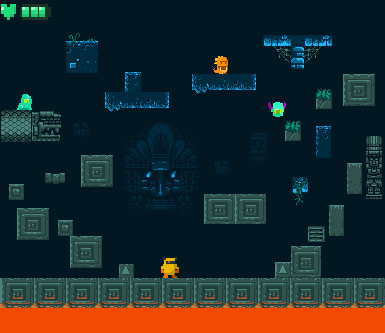
\includegraphics[width=\textwidth, height=14cm]{/home/danhu849/Pictures/game_example.png}}  
\end{figure}

I övre högra hörnet representeras spelarens återstående livspoäng av gröna kuber i en health-bar. Varje nivå i enspelarläge \ref{fig:7} startas med spelkaraktären i nedre delen av spelarfönstret alldeles ovanför lavan. En eller flera utstakade vägar av plattformar i olika höjd placeras över nivån. Slutet på banan representeras ej på bilden ovan då nivån är större i höjdled än spelfönstret.

\newpage
\begin{figure}[h!]
  \caption{LOFI-exempel Tvåspelarläge Nivå start.\label{fig:8}}
  \centerline{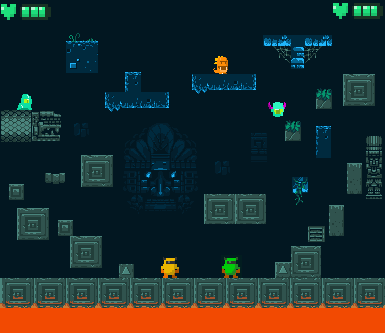
\includegraphics[width=\textwidth, height=14cm]{/home/danhu849/Pictures/game_example_2p.png}}  
\end{figure}
I tvåspelarläge ritas spelarna initialt ut bredvid varandra \ref{fig:8} och lavan aktiveras vid första hoppet från någon av spelarna. Spelare 1s liv representeras i övre vänstra hörnet som vanligt och spelare 2s liv representeras i det övre högra hörnet.

\section{Ska-krav för projektet} % Lägg till referenser till vart respektive krav diskuteras utförligare.
\begin{enumerate}
\item Spelet ska ha en startmeny där spelaren kan välja att starta spelet, visa en nivåmeny, eller avsluta spelet. 
\item I nivåmenyn ska spelaren kunna välja nivå att spela.
\item Varje nivå ska innehålla plattformar.
\item Spelets nivåer ska vara lika breda som spelfönstret och vertikalt större än spelfönstret.
\item Spelaren ska kunna styra en spelarfigur med tangentbordet. % \nameref{tab:1}
\item Spelaren ska ej kunna flytta sig igenom plattformar.
\item Spelaren ska efter första hoppet bli jagad av stigande lava.
\item Spelaren ska dö om den rör lavan.
\item Nivån ska avklaras när toppen nås av spelaren.
\item Nivåns slutpunkt representeras av ett utseendemässigt distinkt område.
\item Efter avklarad nivå ska en meny visas med möjlighet att spela nästa nivå, spela samma nivå igen, eller att gå till startmenyn. 
\item Varje nivå ska innehålla flera instanser av olika typer av fiender.
\item Det ska finnas en flygande fiendetyp  som kan befinna sig mellan plattformar.
\item Det ska finnas en gående fiendetyp som ej förflyttas i höjdled.
\item Fiender ska ej kunna flytta sig igenom plattformar.
\item Alla spelfigurer förutom de flygande fienderna påverkas av gravitation som drar dem nedåt mot spelarfönstrets botten.
\item När spelaren kolliderar med en fiende ska spelarens liv minskas med ett.
\item När spelarens liv minskas ska spelaren inte kunna förlora liv igen under 1.618 sekunder.
\item När spelarens liv når noll ska spelaren dö.
\item Vid spelarens död ska en Game Over meny med möjlighet att starta om eller avsluta nivån visas i spelfönstret.
\item Spelaren ska kunna avfyra projektiler åt det håll spelaren är vänd åt.
\item Projektilerna ska vid kollision med fiender tas bort.
\item Vid kollision mellan spelarens projectiler fiender ska fiendens liv minskat med ett.
\item Projektilerna ska vid kollision med plattformar tas bort.
\item Spelet ska kunna pausas och återupptas genom att tangenten Esc trycks.
\item Det ska finnas en livmätare i spelarfönstret där spelarens återstående liv visas.
\item I spelet ska .csv filer kunna översättas till spelnivåer.
\item Spelets grafik ska vara tvådimensionell.
\item Spelet ska kunna spelas på skolans datorer.
\end{enumerate}

\section{Bör-krav för projektet}

\begin{enumerate}
\setcounter{enumi}{29}
\item Spelarens rörelser ska vara animerade.
\item Fiendernas rörelser ska vara animerade.
\item Projektilernas rörelser ska vara animerade.
\item När en projektil tas bort ska en animerad explosion visas i dess plats. 
\item Lavan ska vara animerad.
\item Två spelare ska kunna spela spelet samtidigt. Spelare ett ges gul färg, spelare två ges grön färg.
\item Spelet ska ha en meny för inställningar där flerspelarläget kan sättas av och på.
\item Det ska finnas en tydligt synlig livmätare i spelarfönstret där spelare 2s återstående liv visas.
\item Spelare 2 ska kunna styra en spelarfigur med en handkontroll.
\item En hoppande fiendetyp ska finnas i spelet.
\item Den hoppande fiendetypen ska kunna avfyra projektiler som färdas i rak bana från avfyrningshöjden.
\item När den hoppande fiendens projektiler kolliderar med spelaren ska spelarens liv minskas med ett.
\item I slutet på en nivå ska det finnas en boss.
\item I bossfighten stoppas lavan vid spelarfönstrets botten.
\item En boss ska ha ett beteende som är skilt från övriga fienders beteenden.
\item En boss ska byta beteende mellan olika spelomgångar.
\item Vilket beteende en boss har ska slumpas fram varje spelomgång.
\item Ljudeffekt ska spelas upp när spelaren skadas.
\item Ljudeffekt ska spelas upp när spelarens projektiler avfyras.
\item Ljudeffekt ska spelas upp när spelare samt fiender dödas.
\item Spelet ska spela bakgrundsmusik.
\item Spelet ska ha en meny för inställningar där musik kan sättas av och på.
\item Spelet ska ha en meny för inställningar där ljudeffekter kan sättas av och på.
\item Spelet ska ha en meny för inställningar där friendly-fire kan sättas av och på.
\item Spelet ska ha en meny för inställningar där kontrollschemat för spelaren kan ändras.
\end{enumerate}



\section{Krav på koden} % Skrivit dem från funktionell synvinkel.
\begin{enumerate}
\item    Spelkoden skrivs i C++17 och ska kunna köras i Ubuntu 20.04.
\item    Koden ackompanjeras med dokumentation.
\item    Det ska ej gå att ändra spelkoden från spelets gränssnitt.
\item    Grafiken ska realiseras med hjälp av SFML.
\item    Koden ska kompileras och köras med en Makefile.
\end{enumerate}

\section{Kravuppfyllelse}

\begin{enumerate}
    \item \textbf{Spelet ska simulera en värld som innehåller olika typer av objekt. Objekten ska ha olika beteenden och röra sig i världen och agera på olika sätt när de möter andra objekt.}
    
    Uppfylls av kraven: 2, 3, 5, 6, 12-17, 21-24, 35, 39-42, 44-46
    
    \item \textbf{Det måste finnas minst tre olika typer av objekt och det ska finnas flera instanser av minst två av dessa. T.ex ett spelarobjekt och många instanser av två olika slags fiendeobjekt.}
    
    Uppfylls av kraven: 5, 12-14, 21, 35, 38, 39, 41
    
    \item \textbf{Ett beteende som måste finnas med är att figurerna ska röra sig över skärmen. Rörelsen kan följa ett mönster och/eller vara slumpmässig. Minst ett objekt, utöver spelaren ska ha någon typ av rörelse.}
    
    Uppfylls av kraven: 13, 14, 21, 38, 39, 41
    
    \item \textbf{En figur ska styras av spelaren, antingen med tangentbordet eller med musen. Du kan även göra ett spel där man spelar två stycken genom att dela på tangentbordet (varje spelare använder olika tangenter). Då styr man var sin figur.}
    
    Uppfylls av kraven: 5, 34, 37
    
    \item \textbf{Grafiken ska vara tvådimensionell.}
    
    Uppfylls av kraven: 28
    
    \item \textbf{Världen (spelplanen) kan antas vara lika stor som fönstret (du kan göra en större spelplan med scrollning, men det blir lite krångligare).}
    
    Uppfylls av kraven: 4
    
    \item \textbf{Det ska finnas kollisionshantering, det vill säga, det ska hända olika saker när objekten möter varandra, de ska påverka varandra på något sätt. T.ex kan ett av objekten tas bort, eller så kan objekten förvandlas på något sätt, eller så kan ett nytt objekt skapas.}
    
    Uppfylls av kraven: 6, 8, 15, 17, 22-24, 41
    
    \item \textbf{ Det ska vara enkelt att lägga till eller ändra banor i spelet. Detta kan exempelvis lösas genom att läsa in banor från en fil.}
    
    Uppfylls av kraven: 27
    
    \item \textbf{Spelet måste upplevas som ett sammanhängande spel som går att spela!}
    
    Uppfylls av kraven: 1-9, 11-26, 29

\end{enumerate}


\end{document}

%%% Local Variables: 
%%% coding: utf-8
%%% mode: latex
%%% TeX-engine: xetex
%%% TeX-master: t
%%% End: 

